
\subsection{Existence as Necessity: The Functional Value of Rock Tokens}

We have observed that \textbf{Rock Tokens} remain resistant to optimization throughout the entire OPD process. To understand the origin of this resistance, we hypothesize that these tokens serve as the structural ``pillars'' of the model's reasoning process. Under this view, the student model may actively protect these tokens from optimization to prevent its internal reasoning framework from collapsing, even when they conflict with the teacher's distribution. This leads to our \textbf{RQ2: Does Rock Token persistence stem from student path dependency?}


\begin{figure}[h]
  \centering
  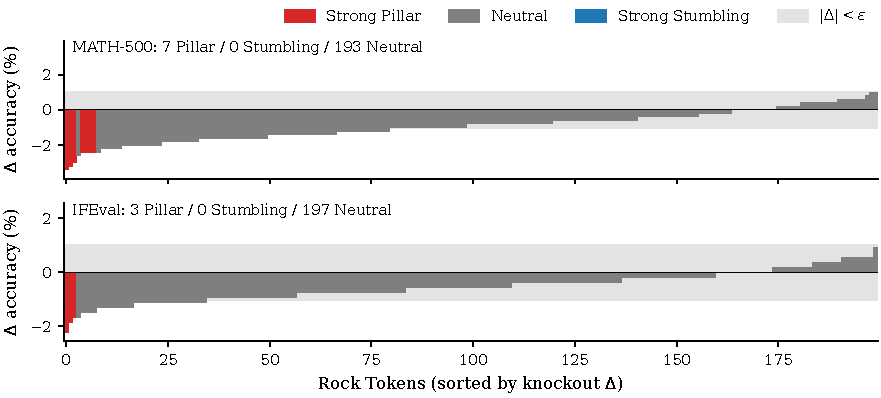
\includegraphics[width=\linewidth]{Figures/Section5/pillar_delta_bar.pdf}
  \caption{\textbf{Knockout effect on the $|\widetilde{\mathcal{R}}|=200$ screened Rock-Token candidates, sorted by $\Delta$.}
  Each bar is a single candidate; height is the accuracy change when its
  logit is masked at decode time. The shaded grey band marks the
  categorization threshold $|\Delta| < \varepsilon = 0.01$. Bars outside the
  band that pass the paired-bootstrap test ($\alpha=0.05$, $10{,}000$
  resamples) are coloured by category (Strong Pillar in red; Strong
  Stumbling in blue). The vast majority of candidates are Neutral on both
  benchmarks; Pillars occupy a short tail and the symmetric Strong-Stumbling
  side is empty --- the visual evidence underlying the sign-asymmetry test
  formalized below.}
  \label{fig:pillar-delta-bar}
\end{figure}
\subsection{Causal Probing via Inference-time Knockout}
\label{sec:knockout_method}

To move beyond distributional metrics and pinpoint the exact functional value of individual tokens, we employ an inference-time \textbf{knockout} procedure. We probe the causal contribution of a token $v$ by observing how its absence affects the model's accuracy on a benchmark $\mathcal{B}$. Specifically, we form a \textit{knockout policy} $\pi_\theta^{\setminus v}$ by forcing the logit of token $v$ to $-\infty$ at every decoding step. We then measure the \textbf{causal delta}:
\begin{equation}
\Delta_{\mathcal{B}}(v) = \mathrm{Acc}_{\mathcal{B}}\bigl(\pi_\theta^{\setminus v}\bigr) - \mathrm{Acc}_{\mathcal{B}}\bigl(\pi_\theta\bigr).
\label{eq:knockout_delta}
\end{equation}
A token $v$ is identified as a \textbf{Strong Pillar} if its removal causes a significant degradation ($\Delta_{\mathcal{B}}(v) \le -0.01$). We screen a pool of $|\widetilde{\mathcal{R}}|=200$ candidates, extending beyond the core $K=100$ set to ensure a wider search for these rare causal effects (see Appendix~\ref{sec:pillar-experiments} for statistical and operational details).

\subsection{Are Rock Tokens Pillars? Findings and Orthogonality}
\label{sec:pillar_findings}

The distribution of $\Delta_{\mathcal{B}}(v)$ in Figure~\ref{fig:pillar-delta-bar} reveals the underlying nature of the Rock Token set. Our investigation yields three primary observations:




\textbf{Pillars are rare but vital:} Only $3.5\%$ of Rock Tokens on MATH-500 and $1.5\%$ on IFEval qualify as Strong Pillars. While most high-KL tokens are neutral residuals, a small subset is absolutely indispensable for the model's reasoning trajectory.
\textbf{Directional Asymmetry:} The complete absence of Strong Stumbling Blocks suggests that the student's "stubborn" deviations from the teacher are rarely detrimental to its own logic; they are either necessary anchors or harmless stylistic preferences.
\textbf{Orthogonality to Traditional Metrics:} 
To examine if Pillarhood can be predicted by standard signals, we analyzed the correlation between $\Delta_{\mathcal{B}}(v)$ and several distributional metrics, including student/teacher entropy, log-frequency, and residual KL. 
Crucially, none of these predictors exhibit a significant correlation with a token's causal importance ($|r| < 0.07$, see Appendix~\ref{sec:pillar-vs-forking} for full analysis and scatter plots). 
This demonstrates that Pillarhood is a property orthogonal to existing importance taxonomies~\cite{tip2026}, suggesting that importance schemes keyed to loss or entropy signals risk suppressing the very tokens the student model cannot reason without.

\begin{takeaway}
\textcolor{tabblue}{\textbf{Take-away}}~
\textbf{The Concentration of Necessity.} 
While Rock Tokens as a population are indispensable for training stability, their causal necessity at inference is highly concentrated: only a tiny fraction ($1.5\%$--$3.5\%$) act as true \textbf{Pillars}. 
This refutes the hypothesis that the student relies on the \textit{entire} high-loss set to maintain reasoning; instead, the model appears to protect a wide "buffer zone" of persistent residuals to ensure a few critical, semantic anchors remain intact.
\end{takeaway}